\chapter[Relatório Lidar]{Relatório Lidar}

O Lidar é uma tecnologia de detecção usado para medição de distâncias ou
outras informações relevantes. O Lidar funciona com a emissão de um laser
que será refletido por um objeto (o que se deseja medir a distância) e depois
detectado fazendo uso das propriedades da luz para se obter as informações
desejadas. Seu funcionamento é parecido com o do radar, porém com pulsos de
laser ao invés de ondas de rádio.


\begin{figure}[h]
  \centering
  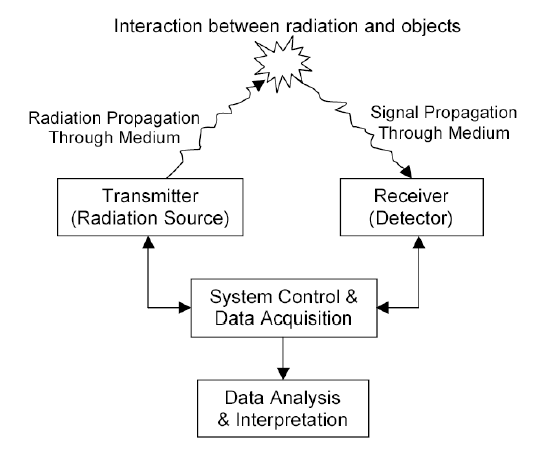
\includegraphics[width=400px, scale=1]{figuras/funcionamento_lidar}
  \caption{Esquemático do funcionamento do Lidar}
\label{fig:funcionamento_lidar}
\end{figure}

\section{Justificativa da escolha}
O Lidar será utilizado no CIAC para medição de diversas distâncias entre carros,
sendo eles os que estão sendo ultrapassados ou os que estiverem na via oposta
durante a ultrapassagem.

	A detecção de luz e o mapeamento com o Lidar é um método preciso para medição
  de referências espaciais e distâncias de objetos, além de fazer uma varredura
  para obtenção dos dados não sendo um detector pontual. O Lidar servirá como um
  sensor para uma maior confiabilidade do sistema CIAC e permite a obtenção de dados
  a partir de ondas eletromagnéticas (o processo físico é extremamente rápido)
  fazendo com que a demora para obtenção da distância entre um carro e outro
  dependa em sua maior parte apenas do processamento desses dados. Uma grande
  precisão em um pequeno intervalo de tempo faz do Lidar uma boa opção
  na utilização do projeto.

	Uma grande desvantagem do Lidar é que sua utilização não é efetiva em
  climas adversos como chuva e neblina devendo ser utilizado em boas condições
  climáticas, na maioria das aplicações com Lidar as detecções são feitas
  de noite onde seu desempenho costuma ser melhor.

\section{ESPECIFICAÇÕES DO LIDAR}

O Lidar utilizado será o HDL-64E da Velodyne que possui uma alta definição e consegue captar uma distância de até 120 m com alta resolução.

Especificações de acordo com a Figura \ref{fig:especificacoes_lidar}

\begin{figure}[h]
  \centering
  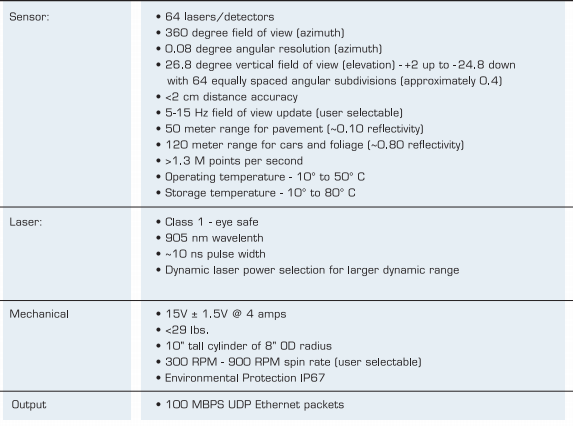
\includegraphics[width=400px, scale=1]{figuras/especificacoes_lidar}
  \caption{Especificações do Lidar}
\label{fig:especificacoes_lidar}
\end{figure}

Design do produto de acordo com a Figura \ref{fig:design_lidar}

\begin{figure}[h]
  \centering
  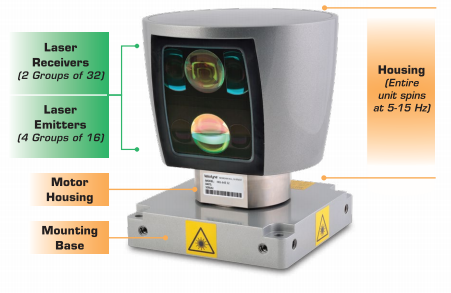
\includegraphics[width=400px, scale=1]{figuras/design_lidar}
  \caption{Design do Lidar}
\label{fig:design_lidar}
\end{figure}
